\documentclass[10pt,twocolumn]{article}
\usepackage[letterpaper,margin=0.72in,columnsep=0.24in]{geometry}
\usepackage{booktabs}
\usepackage{microtype}
\usepackage{graphicx}
\usepackage{pgfplots}
\usepackage{hyperref}
\usepackage{xcolor}
\pgfplotsset{compat=1.18}
\hypersetup{hidelinks,pdfauthor={Anonymous submission},pdftitle={T2424-0027 v3 negative result}}
\setlength{\parindent}{1em}
\setlength{\parskip}{0pt}
\newcommand{\gatefail}{\textbf{FAIL}}
\newcommand{\gatepass}{pass}

\title{Language-Centroid Removal in a Frozen Multilingual Encoder:\\A Preregistered Negative Primary Result}
\author{Anonymous submission}
\date{}

\begin{document}
\maketitle

\begin{abstract}
We tested whether subtracting language-specific centroids from a fixed multilingual sentence representation reduces locale information while preserving intent information more specifically than generic controls. The study was preregistered on a fixed MASSIVE subset with three locales, 50 intents, a pinned multilingual MiniLM encoder, and seeds 2401--2405. The primary rule was a conjunction requiring raw locale accuracy at least 0.75, effect retention at least 0.70, intent drop at most 0.02, specificity margin at least 0.15, and at least four of five seed-level conjunction passes. The retained execution failed that rule: mean raw locale accuracy was 0.492356 (descriptive 95\% Student-$t$ interval 0.480883--0.503828) and the full conjunction passed on 0/5 seeds. Locale centering nevertheless reduced measured locale-probe accuracy to 0.359022 on average and preserved intent accuracy descriptively. Those observations do not rescue the failed preregistered gate. We therefore report a negative primary result with a bounded descriptive finding: under this exact frozen diagnostic, language-centroid removal reduced measured locale leakage while the prerequisite for a strong confirmatory interpretation was not satisfied.
\end{abstract}

\section{Research question and scope}
The narrow question is whether, when a fixed multilingual representation contains measurable locale information, subtracting a fit-split centroid for each locale reduces that information while preserving semantic intent structure more specifically than simple generic controls. This is a representation diagnostic, not a claim about cognition, linguistic relativity, translation quality, universal language invariance, fine-tuned systems, or downstream deployment.

The study uses MASSIVE \cite{fitzgerald2023massive}, but only the preregistered three-locale, 50-intent subset is evidence for the present result. The encoder is a pinned multilingual sentence-transformer from the knowledge-distillation family of Reimers and Gurevych \cite{reimers2020multilingual}; it is not fine-tuned in this study.

\section{Preregistered design}
\paragraph{Data.} The source is \texttt{AmazonScience/massive} at revision \texttt{ff6bd8e4b27c3543e4f8fe2108f32bb95a6f8740}, dataset version 1.1. Locales are exactly \texttt{en-US}, \texttt{es-ES}, and \texttt{fr-FR}. MASSIVE \texttt{train} is the fit split and \texttt{test} is the evaluation split. An outcome-free feasibility census fixed 50 intents with at least 15 examples in every locale and both splits; exactly 15 examples per locale-intent cell were selected in each split by the preregistered SHA-256 ranking rule.

\paragraph{Representation and probes.} The encoder is \texttt{sentence-transformers/paraphrase-multilingual-MiniLM-L12-v2} at revision \texttt{e8f8c211226b894fcb81acc59f3b34ba3efd5f42}, producing 384-dimensional embeddings. The primary probe family is nearest-centroid Euclidean classification fitted only on the fit split. Labels are intent and locale.

\paragraph{Intervention and controls.} Language centering subtracts the fit-split embedding centroid for each true locale. The preregistered controls are global centering, deterministic random-group centering, and deterministic random-subspace removal. Seeds are exactly 2401, 2402, 2403, 2404, and 2405. Seed substitution, favorable-seed reruns, post-outcome intent selection, encoder swapping, control deletion, and threshold movement were prohibited.

\paragraph{Primary gate.} Locale chance accuracy is $1/3$. Normalized language-leakage reduction is
\[
\frac{a_{\mathrm{raw,locale}}-a_{\mathrm{transformed,locale}}}{a_{\mathrm{raw,locale}}-1/3}.
\]
The frozen success rule required all five conditions in Table~\ref{tab:primary}. No $p$-value criterion was preregistered. Intervals reported below were computed post-outcome for description only and cannot replace the conjunction.

\section{Results}
The frozen verdict is \texttt{FAIL\_PREDECLARED\_REAL\_ENCODER\_GATE}. Table~\ref{tab:primary} binds the publication-facing values to the retained result package.

\begin{table}[t]
\centering
\small
\caption{Frozen primary gate. Intervals are descriptive 95\% Student-$t$ intervals across the five frozen seeds and do not alter the gate.}
\label{tab:primary}
\begin{tabular}{@{}lrrl@{}}
\toprule
Quantity & Mean & Frozen rule & Status \\
\midrule
Raw locale accuracy & 0.492356 & $\geq 0.75$ & \gatefail \\
Effect retention & 0.871325 & $\geq 0.70$ & \gatepass \\
Intent drop & -0.002489 & $\leq 0.02$ & \gatepass \\
Specificity margin & 0.816864 & $\geq 0.15$ & \gatepass \\
Seed conjunction & 0/5 & $\geq 4/5$ & \gatefail \\
\bottomrule
\end{tabular}
\end{table}

The decisive failure is the preregistered prerequisite that the raw representation contain strong locale-probe signal. Mean raw locale accuracy was 0.492356, far below the frozen 0.75 floor, and every frozen seed failed the full conjunction. Favorable transformation-specific quantities therefore cannot be promoted into primary success.

\begin{figure*}[t]
\centering
\begin{minipage}{0.49\textwidth}
\centering
\begin{tikzpicture}
\begin{axis}[
width=\linewidth,height=4.3cm,
ybar,bar width=18pt,
ymin=0.28,ymax=0.82,
ylabel={Locale-probe accuracy},
symbolic x coords={Raw,Locale-centered},xtick=data,
error bars/y dir=both,error bars/y explicit,
legend style={font=\scriptsize,at={(0.5,-0.23)},anchor=north,legend columns=2},
tick label style={font=\scriptsize},label style={font=\scriptsize}]
\addplot+[error bars/.cd,y dir=both,y explicit] coordinates {
(Raw,0.492356) +- (0,0.011473)
(Locale-centered,0.359022) +- (0,0.014519)
};
\addplot+[sharp plot,dashed,domain=-1:2] {0.75};
\addplot+[sharp plot,dotted,domain=-1:2] {0.3333333333};
\legend{Retained mean $\pm$ descriptive CI half-width,Preregistered raw floor,Chance}
\end{axis}
\end{tikzpicture}
\end{minipage}\hfill
\begin{minipage}{0.49\textwidth}
\centering
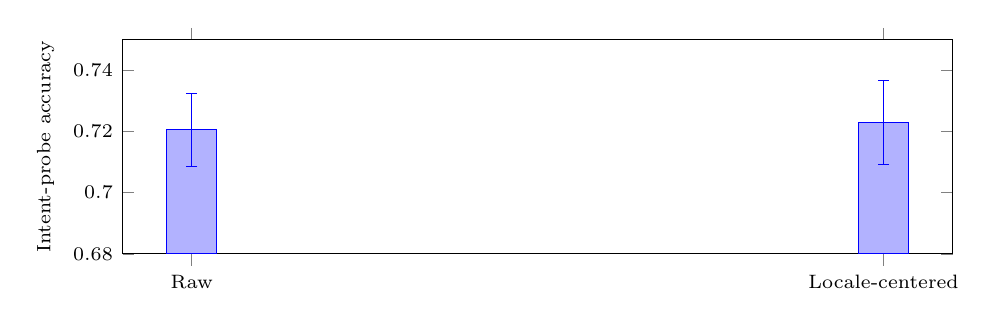
\begin{tikzpicture}
\begin{axis}[
width=\linewidth,height=4.3cm,
ybar,bar width=18pt,
ymin=0.68,ymax=0.75,
ylabel={Intent-probe accuracy},
symbolic x coords={Raw,Locale-centered},xtick=data,
error bars/y dir=both,error bars/y explicit,
tick label style={font=\scriptsize},label style={font=\scriptsize}]
\addplot+[error bars/.cd,y dir=both,y explicit] coordinates {
(Raw,0.720533) +- (0,0.011909)
(Locale-centered,0.723022) +- (0,0.013710)
};
\end{axis}
\end{tikzpicture}
\end{minipage}
\caption{Retained descriptive aggregate outcomes. Left: raw locale-probe accuracy failed the preregistered 0.75 prerequisite; locale centering reduced the measured locale-probe accuracy. Right: intent-probe accuracy was descriptively similar before and after locale centering. Error bars are the retained post-outcome descriptive 95\% Student-$t$ intervals, shown only to summarize seed variability; they are not a rescue criterion or a new significance test.}
\label{fig:descriptive}
\end{figure*}

Language-centered locale accuracy averaged 0.359022 (descriptive interval 0.344503--0.373541), compared with raw locale accuracy 0.492356 (0.480883--0.503828). Mean normalized locale-leakage reduction was 0.835020 (0.732629--0.937411). Raw intent accuracy averaged 0.720533 (0.708624--0.732442), while language-centered intent accuracy averaged 0.723022 (0.709312--0.736732), producing mean intent drop -0.002489 (-0.005501--0.000524).

The specificity margin was 0.816864 (0.718054--0.915674). The preregistered random-group and random-subspace controls produced mean normalized reductions of 0.005157 and 0.008990 respectively, while global centering was 0 under the retained definition. These are descriptive comparisons within the frozen probe pipeline, not evidence that the centering transform is generally optimal.

\section{Interpretation}
The negative primary result is informative because the gate separated two questions that could otherwise be conflated: whether an intervention changes a probe and whether enough target signal existed beforehand to support the intended confirmatory interpretation. Here the intervention changed measured locale recoverability, but the raw locale signal failed the prospectively required floor. The correct conclusion is therefore narrower than the favorable transformation metrics alone might suggest.

The retained evidence supports only the statement that, under this fixed encoder, subset, probe family, and intervention, locale-specific centering produced a large descriptive reduction in measured locale-probe accuracy while intent-probe accuracy was preserved on average. It does not establish complete information removal, downstream benefit, or superiority over stronger concept-erasure methods.

\section{Related work and comparison boundary}
INLP \cite{ravfogel2020inlp} repeatedly trains linear classifiers for a target attribute and projects representations into their null spaces. LEACE \cite{belrose2023leace} gives a closed-form linear concept-erasure transform under its formal assumptions. The present centroid subtraction is substantially simpler and does not inherit their guardedness or minimal-distortion guarantees.

Crucially, INLP and LEACE were not matched baselines in the frozen v3 protocol. Adding either after observing v3 outcomes would be an outcome-responsive protocol change. A direct comparison must therefore be conducted only as a separately preregistered successor study. The present paper makes no state-of-the-art, optimality, or general superiority claim.

\section{Limitations}
Nearest-centroid probe accuracy is only one operationalization of representational information. The evaluation covers exactly three locales and 50 feasibility-filtered intents, not MASSIVE's full language inventory. The encoder is frozen and not fine-tuned. Descriptive intervals summarize only five fixed seeds and were not part of the success rule. Locale centering uses true locale identity and is thus a diagnostic rather than a language-agnostic deployment method. Most importantly, raw locale accuracy failed the preregistered 0.75 prerequisite, directly limiting claims about removal of strong locale information.

\section{Reproducibility and evidence identity}
The retained lineage is protocol \texttt{T2424-0027-REAL-ENCODER-GATE-v3}. The preregistration commit is \texttt{a3fc8fb13c600ec5a7b5a3bc4379b88c80a11c7a}; the preregistration manifest Git blob is \texttt{3adc92ebf9203f20319582e33c98ba570f9d884c}; and the one-shot trigger commit is \texttt{0e9d7c9ad4abd61b8996303fdcd45579b898f327}. The primary retained GitHub Actions execution is run 33307308534, job 99246007605, artifact 9730910606, with retained artifact ZIP SHA-256 \texttt{5bebd21c4e0b763a68c100c58bdea10d1822550d08fcda505ed65c84eb44a757}.

The publication package is fail-closed: it must preserve the negative primary verdict, raw-locale prerequisite failure, 0/5 seed-pass count, and the separation between this real-encoder successor and the earlier synthetic mechanics experiment. Any revised protocol requires a new preregistration.

\section{Conclusion}
The preregistered real-encoder v3 study produced a clear negative primary result. Locale-specific centering substantially reduced measured locale leakage and preserved intent-probe performance descriptively, but raw locale predictability was too weak to satisfy the preregistered prerequisite and no frozen seed passed the full conjunction. Retaining that failure without rescue tuning is the central scientific conclusion.

\begin{thebibliography}{9}
\small
\bibitem{fitzgerald2023massive}
J. FitzGerald et al., ``MASSIVE: A 1M-Example Multilingual Natural Language Understanding Dataset with 51 Typologically-Diverse Languages,'' \emph{ACL}, pp. 4277--4302, 2023. doi: \href{https://doi.org/10.18653/v1/2023.acl-long.235}{10.18653/v1/2023.acl-long.235}.

\bibitem{reimers2020multilingual}
N. Reimers and I. Gurevych, ``Making Monolingual Sentence Embeddings Multilingual using Knowledge Distillation,'' \emph{EMNLP}, pp. 4512--4525, 2020. doi: \href{https://doi.org/10.18653/v1/2020.emnlp-main.365}{10.18653/v1/2020.emnlp-main.365}.

\bibitem{ravfogel2020inlp}
S. Ravfogel, Y. Elazar, H. Gonen, M. Twiton, and Y. Goldberg, ``Null It Out: Guarding Protected Attributes by Iterative Nullspace Projection,'' \emph{ACL}, pp. 7237--7256, 2020. doi: \href{https://doi.org/10.18653/v1/2020.acl-main.647}{10.18653/v1/2020.acl-main.647}.

\bibitem{belrose2023leace}
N. Belrose, D. Schneider-Joseph, S. Ravfogel, R. Cotterell, E. Raff, and S. Biderman, ``LEACE: Perfect linear concept erasure in closed form,'' \emph{NeurIPS}, vol. 36, 2023. doi: \href{https://doi.org/10.52202/075280-2884}{10.52202/075280-2884}.
\end{thebibliography}

\end{document}
